\documentclass[progress]{cmpreport}
\usepackage{natbib}
\usepackage{graphicx}
\usepackage{wrapfig}
\usepackage{paralist}
\usepackage{outlines}
\usepackage{booktabs}
\usepackage{appendix}
\usepackage{float}
\graphicspath{ {./} }

\title{Third Year Project: Progress Report}
\author{Matthew Taylor}
\registration{100151729}
\supervisor{Dr Rudy Lapeer}
\ccode{CMP-6013Y}

\begin{document}

\maketitle

\begin{section}{Introduction}

\subsection{Aim of the project}
The project aims to implement a first person video game which uses procedural generation (PCG) to provide a novel and interesting game experience. The project will explore the technical aspects of using PCG as a core feature of a game, specifically, implementation and performance. 

It will focus on real-time procedural level generation and providing a compelling, dynamic level structure.

\subsection{Motivation}
Procedural generation is not a new field, especially in video games, but there are interesting areas that are seldom explored.

The motivation behind the project's aims are to explore new and interesting concepts, namely, using PCG as a core feature in a game and using real-time procedural generation to provide an interesting experience.
   
\end{section}

\begin{section}{Issues and problems}

\subsection{Project scope}
Procedural content generation is a large field that has been explored in the literature since the 1980s. The paper \cite{Hendrikx:2013:PCG:2422956.2422957} details this, providing a survey of PCG in games and the many techniques that have been used. A potential issue of the project is attempting to explore and implement too many of these techniques and ending up with a dilted project of little technical interest. 

To avoid this, the project scope was focussed on some areas identified as being under explored in the survey - level generation in real time systems. This will allow the project to explore several ideas in this domain and provide a comprehensive implementation in a fully featured game.

\subsection{Designing 3D games}
Designing 3D games and the assets required to populate the levels created could take a long time, especially if much of the functionality is created from scratch. To enable the project's aims to be achieved in a realistic timeframe, the Unity game engine was chosen. This tool enables relatively rapid production 3D game enviroments, supporting the design of assets and enabling quick prototyping of ideas. Unity supports the use of C\# as a scripting language to program game features in. It also provided a lot of documentation, which was useful in learning the framework and the systems it provides. Much of the initial stages of the project focussed on learning Unity.

\subsection{Performance}
A game's performance is a critical aspect of it's success. If the game cannot be played in a sustainable framerate on common hardware, it could be considered a techncial failure. The prototype stage considered performance at every aspect, in two ways.

One performance issue could be \textbf{level generation speed}. Each time the game loads, a new level is generated, so achieving a suitable speed in generating the levels and performing the associated work, like loading geometry, was a key consideration.

Another could be \textbf{framerate}. The project will procedurally load a considerable amount of geometry in varied conditions. As much of the geometry will not be static, it will be required to load a large amount of meshes into memory, which could affect the performance.  

\subsection{Evaluation of success} \label{evalsuccess}
A key issue with this project is evaluating if it is successful. If there is no clear notion of what success looks like, the project could progress in unproductive directions. Below are the key measures of success chosen at the start of the project to measure success against.

\subsubsection{Convincing levels}
The levels must appear convincing. This is difficult to quantify, but nevertheless is an important attribute. The levels (at least in the initial design) will be mazes generated in a grid, with the grid sections subdivided in different ways.

This could easily create a boring level, where the grid pattern is discernable and the rooms are boring and procedural to traverse. Successful generation of levels will avoid these issues.

\subsubsection{Convincing decoration}
The decoration in each individual room will contribute to how convincing and hand-crafted each level looks. As described in \cite{doi:10.1111/j.1467-8659.2009.01351.x} and \cite{taylor-parberry}, there are several challenges to making room decoration appear to be hand-made when it is procedurally generated. 

Of particular focus will be generating furniture and objects in and around that furniture that is generated, but remains plausable. To use this as a measure of success in the project, attention will be paid to the interior decoration being unique in each room, yet also being plausable (ie. no bookcases facing walls, chairs in doorways, etc.)


\subsubsection{Performance}
Performance is another key component of the project succeeding. If the game responds poorly, it will be frustrating to play. Performance will be measured in a few ways:
\newline
\begin{compactitem}
    \item{\textbf{Frame rate}: must be at least 30 frames per second}
    \item{\textbf{Initial loading time}: must take less than 30 seconds}
    \item{\textbf{Smooth level re-generation}: no dip in framerate}
\end{compactitem}



\end{section}

\begin{section}{Design and planning}

\subsection{Implementation methodology}
The project development operates under an Agile methology. Agile does not require that all requirements (or "user stories") are defined up front, instead it is encouraged that they are developed and refined during the lifecycle of the project.

The project itself is divided into Agile "sprints". It was decided to deliver a sprint every two weeks, as this fit with the development time given to the project and providing updates to the project supervisor.

While all the stories were not required at the outset, as part of the planning, it was decided to plot rough timescales against Agile "epics". These epics provide a high-level view of functionality and are detailed in Table \ref{tab:epics} on page \pageref{tab:epics}.

The epics also contain very high-level user stories, which provide a little more detail. These were decided at the project outset, then refined during development. Before any user story can be developed, it is required that more detailed requirements are written. These are then recorded and tracked on Trello. 

\subsection{Implementation plan}

With the high-level design documented in the epics, planning of these epics against timescales was required. This timeline plan is visible in \ref{fig:gantt1} on page \pageref{fig:gantt1}. Progress was then tracked against this Gantt chart to ensure that progress was being made and that the project could be achieved as planned.

As the project is run using Agile principles, the Gantt chart has been revised to reflect changes to the plan. These changes are visible in Figure \ref{fig:gantt2} on page \pageref{fig:gantt2}. Also included is the progress of the tasks so far.

Changes to the Gantt chart include the addition of a Level Generation task - the Level Re-Generator. This reflects a focus of the project on procedurally re-generating levels in real-time, so this has been split out as a seperate task and given a shorter timescale, reflecting the importance of the task to the project.

The gameplay section has been split into two tasks, reflecting the focus on implementing core gameplay as a priority, with enhanced gameplay being desirable but not as critical to the evaluation of success of the project.


\subsection{UML}

As the project began, a UML diagram was designed to provide a high level framework to work towards. Unity provides some pre-defined structure, in that all game objects must be part of a Scene object to work. Aside from this, Unity does not prescribe much structure, so a UML design to begin with was useful. The initial UML design can be seen in Figure \ref{fig:uml1} on page \pageref{fig:uml1}.

This design was iterated upon as the prototype stage progressed. This can be seen in Figure \ref{fig:uml2} on page \pageref{fig:uml2}, which shows the definition of classes being enhanced with the additional methods and attributes required to support the design, as well as the addition of the \textbf{Level Re-Generator} class.


\subsection{Requirements and prioritisation}

\subsection{Design}
\subsubsection{Guaranteed path generation}
The first part of the design to be implemented required a guaranteed path through a maze to be generated. This was achieved by using a random walk - a stochastic process implmented in two dimensions to provide a definite route through the maze.

The random walk is implemented using an agent based approach. The agent can choose from three random directions to travel in - left, right or down. These probabilities are detailed in Table \ref{tab:probdirs}.



This skewed probability distribution encourages the path generating agent to meander left and right more than moving down, generating a path that is longer and doubles back on itself more.



\end{section}

When the agent has chosen a valid direction, it randomly selects a valid tile. To aid in creating an interesting maze, the agent can choose from a variety of pre-made tiles with varying exits. For example, it may choose to generate a room with only left and right openings, or a tile with openings on the left, right and down-facing aspects. 

The agent has methods of checking where it has been and where it is going next, so that it picks valid tiles that have openings in the directions it has come from and intends to go.

The agent is given bounds and restrictions while it is performing the random walk. These bounds ensure the generation does not stray too far left or right. When the agent reaches the lowest down-bound, it stops generating the level and spawns the level's goal in the final tile it generated.

These bounds are adjusted by parameters, which aid in development and testing and can be adjusted based on performance or desired level size.



\begin{section}{Evaluation of progress}

\subsection{Progress against plan}
As detailed in the revised Gantt chart in Figure \ref{fig:gantt2} on page \pageref{fig:gantt2}, progress is broadly on plan. The prototyping of the level and room generation is complete and suitable methods have been implemented. Much of the remaining work on level and room generation will focus on refining the performance, achieving higher levels of complexity and improving performance.

\subsection{Changes to plan}
The plan has changed slightly since the project began. As can be seen in the differences between Figure \ref{fig:gantt1} and Figure \ref{fig:gantt2} on page \pageref{fig:gantt2}, two new tasks have been added.

The \textbf{Level Re-generator} task has been added and given a shorter timeframe to provide focus on this task. The re-generation aspect of the project is important to consider when evaluating performance It also provides a novel feature not seen in many computer games, so this was considered important to focus on.

The \textbf{Add Enhanced Gameplay} task was also added, to provide a marked difference between the basic implementation and a more detailed gameplay experience. It will not require much effort to provide a basic experience, which will be important to implement early. The project will then consider enhanced gameplay elements (more enemies, pickups, keys for locked doors) towards the end of the project, after the main aims have been achieved.

\subsection{Evaluation against success measures}
In Section \ref{evalsuccess} on page \pageref{evalsuccess}, three measures of success for the project were defined. 

Against the \textbf{Convincing Levels} measure, the project has the potential to succeed. The guaranteed path/tile filling combination creates large levels, with a path through them. The project does not currently take steps to block off many of the non-guaranteed path tile transitions, so the tile structure is disernable - it is quite easy in parts to see how the tiles are laid out. Future 

\end{section}






\bibliography{sources}

\newpage

\appendix

\begin{section}{Gantt charts}

\begin{figure}[H]
    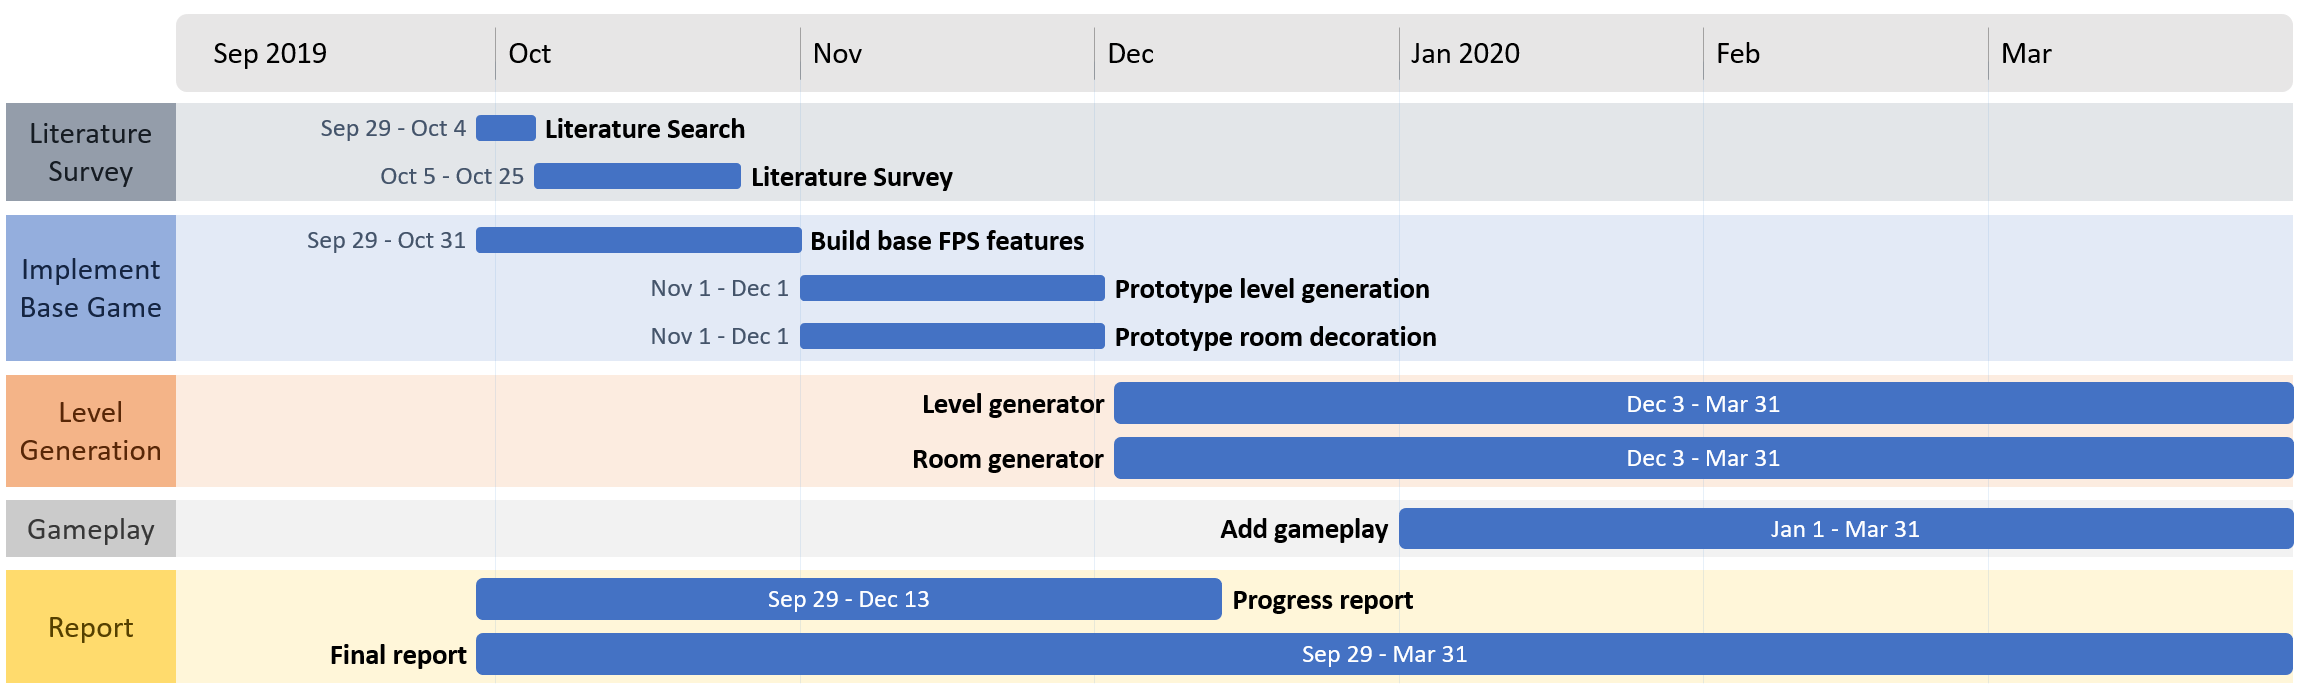
\includegraphics[width=\textwidth,height=0.9\textheight,keepaspectratio]{img/gantt-original.png}
    \caption{Gantt chart of original plan}
    \label{fig:gantt1}
\end{figure}

\begin{figure}[H]
    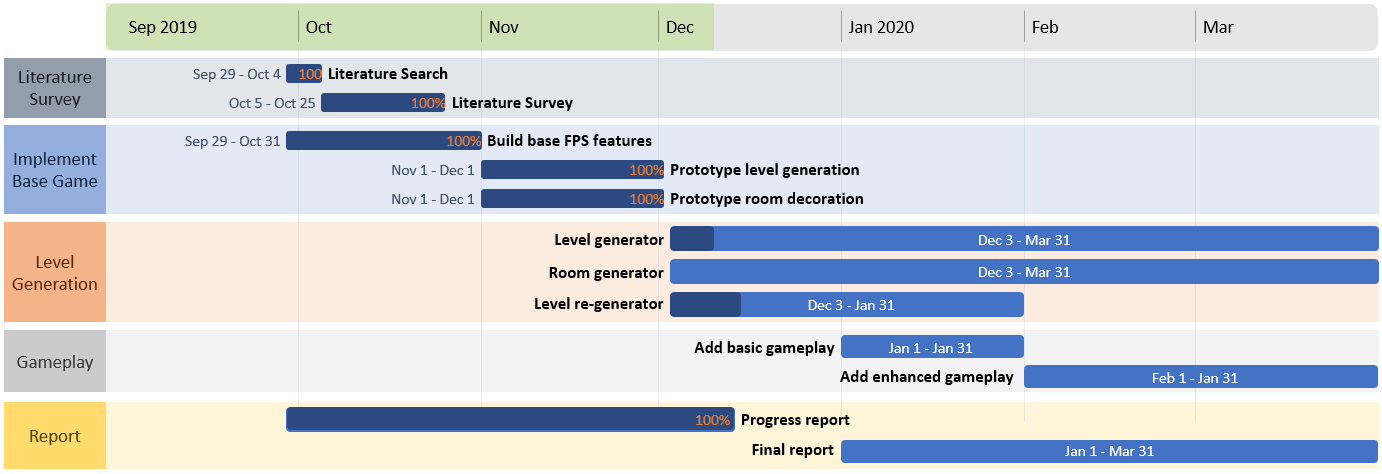
\includegraphics[width=\textwidth,height=0.9\textheight,keepaspectratio]{img/gantt-updated.png}
    \caption{Gantt chart of updated plan}
    \label{fig:gantt2}
\end{figure}

\end{section}

\begin{section}{Diagrams}

\begin{figure}[H]
    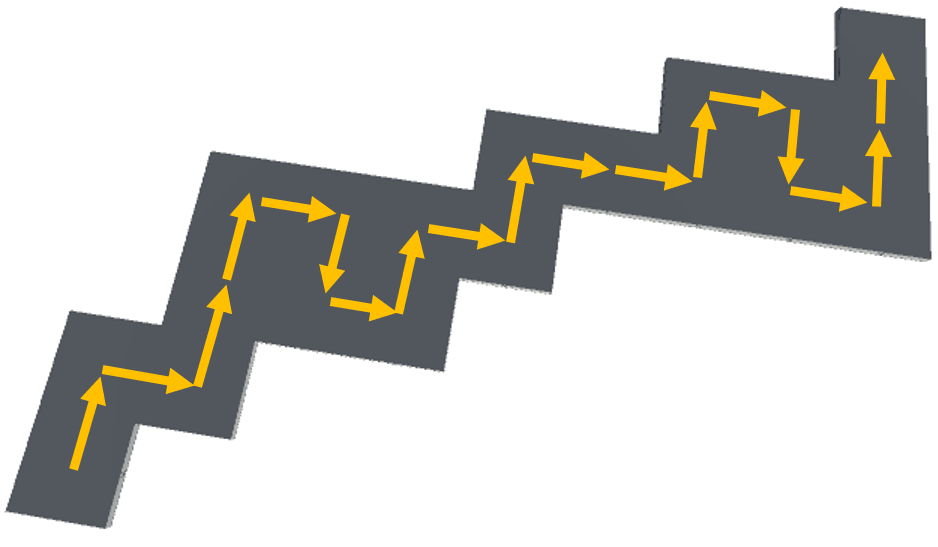
\includegraphics[width=6cm]{img/1-maze.png}
    \caption{A top-down view of the guaranteed path generation}
    \label{fig:pathgen}
\end{figure}

\begin{figure}[H]
    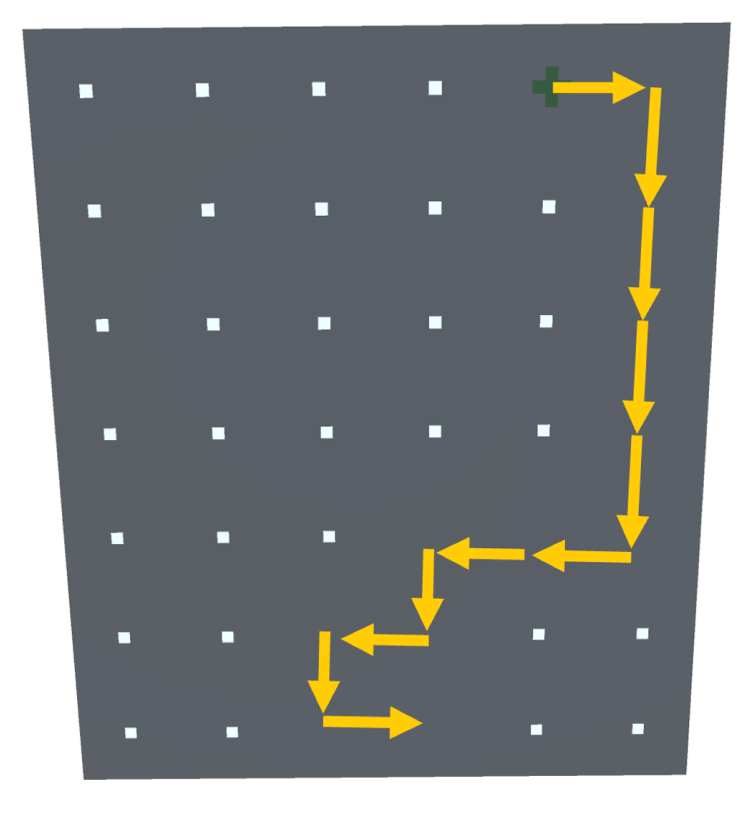
\includegraphics[width=6cm]{img/filled-path.png}
    \caption{A top-down view of the guaranteed path with remaining tiles filled in}
    \label{fig:filledpath}
\end{figure}



\begin{figure}[H]
    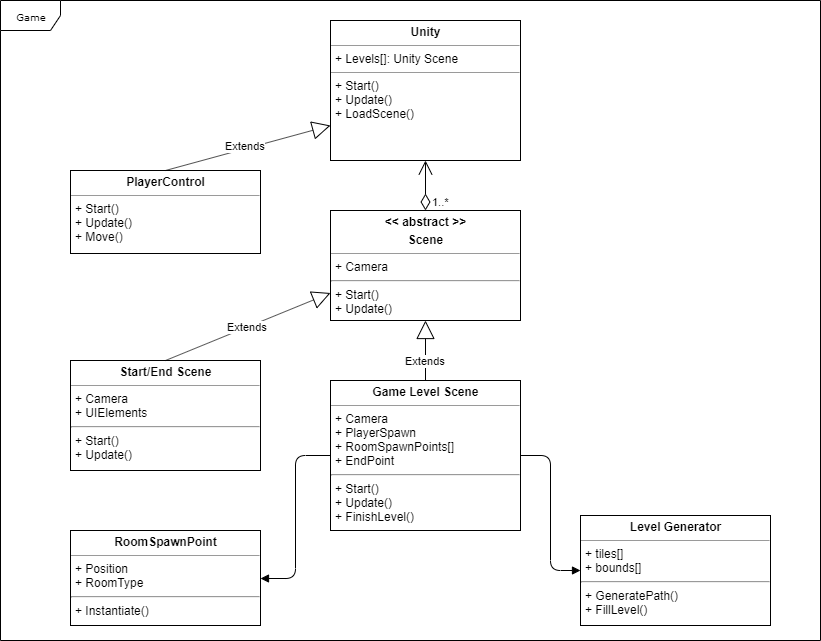
\includegraphics[width=\textwidth]{img/uml1.png}
    \caption{Initial UML diagram}
    \label{fig:uml1}
\end{figure}

\begin{figure}[H]
    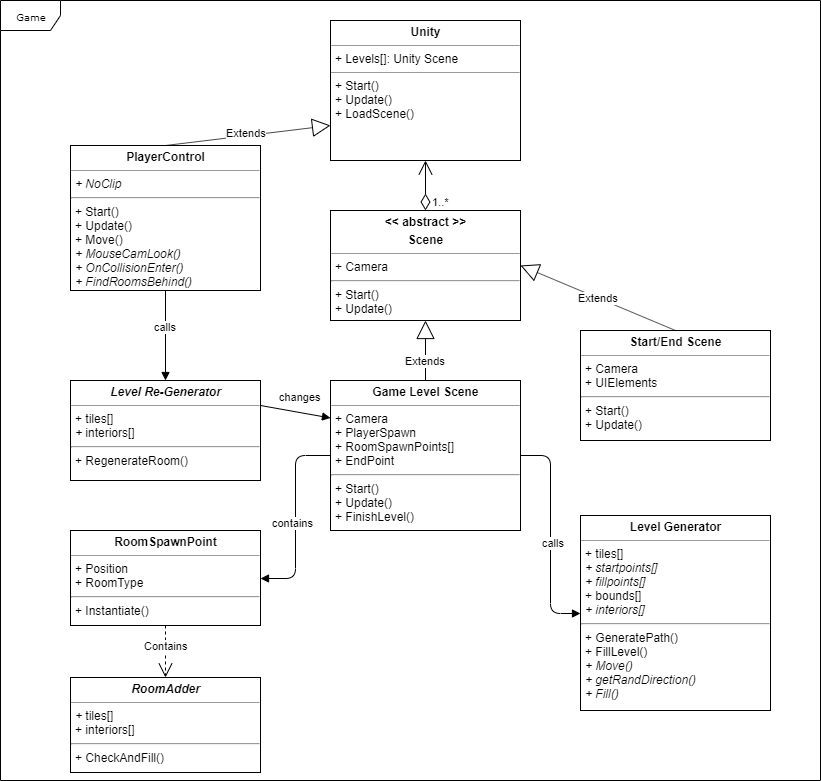
\includegraphics[width=\textwidth]{img/uml2.png}
    \caption{Redesigned UML diagram}
    \label{fig:uml2}
\end{figure}

\end{section}

\begin{section}{Tables}

% epic/story table
\begin{table}[]
    \resizebox{\textwidth}{!}{%
    \begin{tabular}{@{}ll@{}}
    \toprule
    \multicolumn{1}{l|}{\textbf{Epic}} & \textbf{Stories} \\ \midrule
    \multicolumn{2}{l}{Build base "first person" 3D game features} \\
     & Provides a basic level design \\
     & Proves the concepts of vision and movement \\ \midrule
    \multicolumn{2}{l}{Prototype level generation} \\
     & Prove a method of generating a guaranteed path through a maze \\
     & Prove a method of filling in non-guaranteed paths through the maze \\ \midrule
    \multicolumn{2}{l}{Prototype room generation} \\
     & Prove a method of generating room interiors \\
     & Room generation must not interfere with guaranteed path \\ \midrule
    \multicolumn{2}{l}{Prototype level re-generation} \\
     & Design method to procedurally re-generate level sections \\ \midrule
    \multicolumn{2}{l}{Add gameplay elements} \\
     & Decide on how level is finished by the player \\
     & Provide some interest and threat when playing \\
     & Provide means of assisting navigation \\ \midrule
    \multicolumn{2}{l}{Implement final designs} \\
     & Use non-prototype textures \\
     & Ensure performance meets goals \\ \bottomrule
    \end{tabular}%
    }
    \caption{Agile-style epics and associated user stories}
    \label{tab:epics}
\end{table}

\begin{table}[h!]
    \centering
    \begin{tabular}{ |c|c|c| }
    \hline
    Left & Right & Down \\ 
    \hline
    40\% & 40\% & 20\%\\ 
    \hline
    \end{tabular}
    \caption{A table showing probability of direction random walk agent will take}
    \label{tab:probdirs}
\end{table}

\end{section}

\end{document}
